%chktex-file 1 %chktex-file 3 %chktex-file 8 %chktex-file 9 %chktex-file 10 %chktex-file 11 %chktex-file 12 %chktex-file 13 %chktex-file 16 %chktex-file 17 %chktex-file 18 %chktex-file 25 %chktex-file 26 %chktex-file 35 %chktex-file 36 %chktex-file 37 %chktex-file 40 %chktex-file 44 %chktex-file 45 %chktex-file 49
\section{Теорема Жордана}
    Основное условие: \ \  $\phi: \ V \to V$ - линейный оператор, все его корни $\in \F$
    $$\chi_{\phi}(\lambda) = (-1)^n(\lambda-\lambda_1)^{k_1}\cdot\ldots\cdot(\lambda-\lambda_s)^{k_s} \ (\forall i\neq j: \ \lambda_i\neq\lambda_j \text{ и } \sum \limits_{i=1}^s k_i = \dim V)$$
    $$V = K_1\oplus\ldots\oplus K_s, \ \text{где } K_i = \text{Ker}(\phi-\lambda_i\cdot\text{id})^{k_i} - \text{корневое подпространство}$$
    $$V_{\lambda_i} = \{x\in V \ | \ \phi(x) = \lambda_ix\}, \  \dim V_{\lambda_i}\leqslant k_i = \dim K_i$$
    Так как $K_i$ - инвариантное подпространство относительно оператора $\phi$, можно рассмотреть ограничение: 
    $$(\phi-\lambda_i \text{ id})|_{K_i} := B_i$$
    Из определения $K_i$ следует, что $B_i^{K_i}=0$, то есть $B_i$ - нильпотентный оператор.\\
    %Обозначим $h_i$ - показатель нильпотентности оператора, т.е. $B_i^{h_i}=0$,\\ 
    %но $B_i^k\neq0$ $\forall k < h_i$\\
    В базисе, согласованном с этим разложением: 
    $$A_{\phi} = \begin{pmatrix}
    \text{\fbox{$A_1$}}\\
    \null & \text{\fbox{$A_2$}}\\
    \null & \null & \ddots\\
    \null & \null & \null & \text{\fbox{$A_s$}}
    \end{pmatrix}$$
    где $A_i = A_{\phi_{k_i}}$ - матрица порядка $k_i, \  A_i-\lambda_iE_{k_i} = B_i, \ B_i^{k_i}=0$\\
    Обозначим $K_i :=K$, $B_i :=B$, $k_i :=k$, тогда: 
    $$\forall x\in K: \  B^k(x) = 0$$
    если $x\neq0$, то $\exists$ наименьшее значение $m$: 
    $$B^m(x) = 0, \ B^{m-1}(x)\neq 0 \ (m\leqslant h)$$ 
    Назовём это высотой вектора $x$.\\
    Для фиксированного вектора $x\neq0$ (высоты $m$) рассмотрим векторы: 
    $$x, \  Bx, \ldots,B^{m-1}x, \ B^mx = 0$$
    \begin{definition}
        Векторы \{$x,\ Bx,\ \ldots,\  B^{m-1}x $\} называются жордановой цепочкой.
    \end{definition}  
    \begin{lemma}
        Вышеуказанные векторы являются линейно независимыми.
    \end{lemma}
    \begin{proof}
        Предположим, что: 
        $$\alpha_0x+\alpha_1Bx+\ldots+\alpha_{m-1}B^{m-1}x=0$$
        Подействуем на это равенство оператором $B^{m-1}$: $$\alpha_0B^{m-1}x = 0 \ \Longrightarrow \ \alpha_0 = 0$$ 
        На оставшиеся векторы подействуем оператором $B^{m-2}$:
        $$\alpha_1B^{m-1}x = 0 \ \Longrightarrow \ \alpha_1 = 0$$
        и т.д. Получим, что $\forall i = \overline{0,m-1}: \ \alpha_i = 0 \ \Longrightarrow$ векторы являются линейно независимыми.
    \end{proof}
    \begin{definition}
        Подпространство, натянутое на эти векторы: $$\langle x,\ Bx,\ \ldots,\  B^{m-1}x \rangle$$
        называется циклическим подпространством, порождённым жордановой цепочкой. Данное подпространство обозначим $U_x$, $\dim U_x = m$.\\
        Обычно векторы жордановой цепочки нумеруют с конца, то есть:
        $$a_1 = B^{m-1}x, \ a_2 = B^{m-2}x, \ldots, a_m = x$$ 
        Тогда $a_1$ - собственный вектор для $B$, и для $\forall j = \overline{2,m}: \ a_{j-1} = Ba_j$.\\
        Вектор $a_j$ называется \textbf{присоединённым} к вектору $a_{j-1}$.\\
        К вектору $a_1$: \ $a_2$ - присоединённый, $a_3$ - второй присоединённый и т.д. 
    \end{definition}
    \begin{definition} $\\$ 
        Матрица ограничения оператора $B$ на подпространство $U_x = \langle a_1\ldots a_m\rangle$ : 
        $$B|_{U_x} = \begin{pmatrix}
        0 & 1\\
        \null & 0 & 1\\
        \null & \null & \ddots & \ddots\\
        \null & \null & \null & 0 & 1\\
        \null & \null & \null & \null & 0
        \end{pmatrix} = J_k(0)$$ 
        называется жордановой клеткой с собственным значением $\lambda = 0$
        $$\lambda=\lambda_i: \ A_{\phi|_{U_x}} = \begin{pmatrix}
        \lambda_i & 1\\
        \null & \lambda_i & 1\\
        \null & \null & \ddots & \ddots\\
        \null & \null & \null & \lambda_i & 1\\
        \null & \null & \null & \null & \lambda_i
        \end{pmatrix}=J_k(\lambda_i)$$ 
        - жорданова клетка с собственным значением $\lambda = \lambda_i$, где: 
        $$\phi(a_2) = a_1+\lambda_ia_2, \ \phi(a_{j+1}) = a_j+\lambda_ia_{j+1}$$
    \end{definition} 
    Перед доказательством теоремы докажем лемму:
    \begin{lemma}
        Если $B$ - такой оператор в пространстве $V$, что: 
        $$\text{Im}B = B(V) \subset V$$
        то $V$ обладает $(n-1)$-мерным инвариантным подпространством $W$, таким что $\textup{Im}B \subseteq W$.
    \end{lemma}
    \begin{proof}
        Пусть $e_1,...,e_m$ - базис в $\text{Im}B, \ m<n = \dim V$\\
        Дополним его до базиса в $V$ векторами $e_{m+1},...,e_n$.\\
        Тогда $W = \langle e_1,...,e_{n-1} \rangle$ - искомое инвариантное подпространство:
        $$\forall w = \sum \limits_{i=1}^{n-1}\beta_ie_i \Longrightarrow Bw = \sum \limits_{i=1}^{n-1}\beta_iBe_i \in \text{Im}B \subseteq W$$
    \end{proof}
    %\begin{lemma}
    %    Если $U = \langle e, \ Be,\ ...,B^{m-1}e \rangle$, то:
    %    $$\forall y \in U \ \exists \ f(t) \in \F[t]: \ y = f(B)e, \ \deg f \leq m-1$$
    %    Если $f(0) \neq 0$, то высота $y = m$, то есть $y$ порождает то же циклическое подпространство.     
    %\end{lemma}
    %\begin{proof}
    %    Очевидно из определения линейной оболочки.
    %\end{proof}
    \begin{theorem} \textbf{Жордана} \\
        \tab[0.5cm]Если все характеристические корни опертора $\phi: \ V \to V$ принадлежат полю $\F$, то $V$ является прямой суммой циклических подпространств для оператора $\phi$. Это равносильно тому, что в $V$ существует базис, составленный из жордановых цепочек. Такой базис называется жордановым базисом.\\
        \tab[0.5cm]Если жорданов базис уже построен: Пусть имеются $r$ жордановых цепочек, отвечающих собственным значениям $\lambda_1, \ldots, \lambda_r$, необязательно различным, длины которых $m_1,\ldots,m_r$ соответственно, тогда в этом базисе:
        $$A_{\phi} = \begin{pmatrix}
        \text{\fbox{$J_{m_1}(\lambda_1)$}} & \null & \null & 0 \\
        \null & \text{\fbox{$J_{m_2}(\lambda_2)$}}\\
        \null & \null & \ddots\\
        0 & \null & \null & \text{\fbox{$J_{m_r}(\lambda_r)$}}\\
        \end{pmatrix} \ \ \ \sum \limits_{i=1}^rm_i = n = \dim V$$ 
        - жорданова матрица - жорданова нормальная форма (ЖНФ) матрицы $A_{\phi}$.
    \end{theorem}
    \begin{theorem}\textbf{Жордана (матричная формулировка)} \\
        Для любой матрицы $A \in M_n(\F)$, все характеристические корни которой $\in \F$, $\exists$ матрица $C \ (\det C \neq 0)$ такая, что: 
        $$C^{-1}AC = J$$
        - жорданова матрица. При этом жордановы клетки определены для матрицы $A$ единственным образом с точностью до расположения клеток на диагонали жордановой матрицы.  
    \end{theorem}
    \begin{remark}
        Матрицу $A$ можно интерпретировать как матрицу линейного оператора $\phi$, для него верна теорема Жордана.  
    \end{remark}
    \begin{proof} (См. Шафаревич И.Р. "Линейная алгебра")\\
        Доказательство достаточно провести для ограничения оператора на каждое корневое подпространство $K_i$.\\ 
        Введем обозначения: $B: \ V \to V$ - нильпотентный оператор, $\dim V = n, \ W - (n-1)$-мерное инвариантное подпространство в $V$, содержащее $\textup{Im}B$  (существует по лемме 1).

        Докажем теорему индукцией по $n$:\\
        База: если $n=1$, то $B = 0$ и любой базис - жорданов.\\
        Пусть $n>1$, тогда по предположению индукции в $W \ \exists$ базис для $B|_w$, т.е.
        $$W = U_1 \oplus ... \oplus U_r$$
        Выберем вектор $a \in V\setminus W$, тогда $a$ ЛНЗ с векторами из $W$.\\
        Рассмотрим $Ba \in W$ (т.к. $\textup{Im}B \subseteq W$) так, что $Ba = u_1 + ... + u_r, \ u_i \in U_i \ (*)$. \\
        Если $Ba = 0$, то:
        $$V = \langle a \rangle \oplus U_1 \oplus ... \oplus U_r - \text{искомое разложение пространства}$$
        Если $Ba \neq 0$, то найдется $i$, что $u_i \neq 0$.\\
        Если в разложении есть $u_i \in B(U_i)$, то  $\exists \ v_i \in U_i: \ u_i = Bv_i$.\\
        Рассмотрим вместо $a$ вектор $a-v_i: \ B(a-v_i) = u_1 + ... + \not u_i+...+u_r - \not u_i \Longrightarrow $ в разложение такого вектора $u_i$ не входит.\\
        Заменив $a$ на нужные разности $a-v_i$, получим новый вектор $e \in V\setminus W$, при этом занулив все $u_i \in B(U_i)$, т.е.
        $$Be = u'_1 + ... + u'_r, \ \forall i \text{ либо } u'_i \not \in B(U_i), \text{ либо } u'_i = 0$$
        Хотя бы один из векторов $u'_i \neq 0$, выберем из них вектор, имеющий максимальную высоту $m$. Заметим, что $m=\max (\dim U_i)$, так как каждый $u'_i$ по построению нового разложения имеет максимальную высоту в своём подпространстве. Тогда $h(e) = m+1$, т.к. $h(Be) = m$. \\
        Без ограничения общности выбрали вектор $u_1$. Докажем, что:
        $$V = \langle e, \ Be, \ ..., \ B^me \rangle \oplus U_2 \oplus ... \oplus U_r$$
        Сумма размерностей подпространств в правой части: 
        $$(m_1+1)+...+m_r = n = \dim V$$
        Поэтому для прямой суммы достаточно доказать, что: 
        $$\langle e, \ Be, \ ..., \ B^me \rangle \cap (U_2 \oplus ... \oplus U_r) = \{0\}$$
        Пусть $v = \lambda_1 e +...+ \lambda_{m+1}B^me \in U_2 \oplus ... \oplus U_r$ \\
        Т.к. $e \not \in W$, $\lambda_1 = 0$. $Be = u'_1+...+u'_r \Rightarrow$ проекция $Be$ на $U_1$ равна $u'_1$.\\
        Спроецируем всё разложение на $U_1$: 
        $$\lambda_2u_1+\lambda_3Bu_1+...+\lambda_{m+1}B^{m-1}u_1 = 0 \Longrightarrow \lambda_2=...=\lambda_{m+1} = 0 \Longrightarrow v = 0$$   
        Существование ЖНФ доказано. Доказательство единственности приводится в следующем пункте.   
    \end{proof}
    \begin{remark}
        $r$ - количество циклических подпространств в разложении корневого подпространства $K$, отвечающего корню $\lambda_0$, равно геометрической кратности корня $\lambda_0$ характеристического многочлена.    
    \end{remark}


    \subsection{Изображение разложения корневых подпространств}
    Обозначим: $r = \dim \text{Ker}B$ - размерность собственного подпространства\\
    Занумеруем собственные векторы, входящие в цепочки, располагая цепочки по убыванию высоты. $m$  - максимальная высота цепочки, $1$ - минимальная\\
    Также введем обозначение для последовательных присоединённых векторов: есть $p_1$ цепочек высоты $m$, \ $p_2$ - высоты $m-1$,..., $r-(p_1+...+p_{r-1})$ - высоты $1$
    \begin{center}
        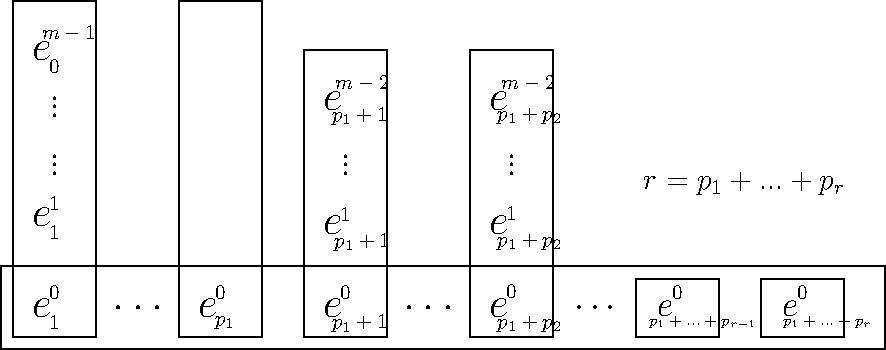
\includegraphics[width=15cm]{image/Asymptote/1/linal-1-1.pdf}
    \end{center}
    $V = U_1 \oplus ... \oplus U_r, \ \dim U_{i+1}\leq \dim U_i$
    \begin{center}
        $BV = BU_1 \oplus ... \oplus BU_r$\\
        $\vdots \tab[4cm]$ \\ 
        $B^kV = B^kU_1 \oplus ... \oplus B^kU_r$  
    \end{center}
    Если $\dim U_i = m_i, \ \dim (B^kU_i) = \left[\begin{matrix}
        m_i - k, \ \text{если } k<m_i\\
        0, \ \text{если } k\geq m_i
    \end{matrix} \right. \Longrightarrow$
    $$\dim (B^kV) = \sum \limits_{i=1}^r \dim B^kU_i = q_{k+1}+2q_{k+2} + ... + (m-k)q_m$$ 
    Пусть $q_i$ - число циклических подпространств размерности $i$, \ $1\leq i \leq r$\\
    Обозначим $r_k = \text{rk}B^k$\\
    Для $k = 0$ до $m-1$ получим равенства: 
    \begin{center}
        $k=0: \ q_1 + 2q_2 + ... + mq_m = n\tab[2.9cm]$\\
        $k=1: \ q_2 + 2q_3 + ... + (m-1)q_m = r_1 = \text{rk}B$\\
        $\cdots$\\
        $q_m = r_{m-1} = \text{rk}B^{m-1} \neq 0$ \\
        $B^m = 0$ на корневом подпространстве     
    \end{center}
    Вычитая из каждого уравнения следующее, получим систему:
    $$\begin{cases}
        q_1 + q_2 + ... + q_m = n - r_1 \tab[0.13cm] \Longrightarrow q_1 = n - 2r_1 + r_2 \\
        \tab[1.05cm] q_2 + ... + q_m = r_1 - r_2 \Longrightarrow q_2 = r_1 - 2r_2 + r_3\\
        \tab[3.5cm]\cdots\\
        \tab[6.9cm]q_m = r_{m-1} - r_m \ (r_m = 0)
    \end{cases}$$
    $$\Longrightarrow q_i = r_{i-1} - 2r_i + r_{i+1} \ (i = 1,...,m-1)$$
    Вывод: количество и порядок (высоты цепочек) однозначно опреледяется по матрице $B=A|_{\phi-\lambda \text{id}}$ - эти ранги не зависят от конкретного разложения $\Longrightarrow$ определяются единственным образом, т.е. \textbf{ЖНФ единственна с точностью до перестановки клеток на диагонали}.
    \begin{consequense}
        Пусть: 
        $$\chi_\phi = (-1)^n(\lambda-\lambda_1)^{k_1}\cdot ... \cdot (\lambda-\lambda_s)^{k_s}$$
        - характеристический многочлен
        $$\mu_\phi = (\lambda-\lambda_1)^{m_1}\cdot ... \cdot (\lambda-\lambda_s)^{m_s}$$
        - минимальный многочлен\\
        Тогда $\forall i = \overline{1,s}: \ m_i$ равна $\max$ размерности жордановой клетки, отвечающей корню $\lambda_i$   
    \end{consequense}
    \begin{consequense}\textbf{ Критерий диагонализируемости в терминах min многочлена:} \\
        Оператор $\phi$ диагонализируем $\Longleftrightarrow m_1 = ... =m_s=1$  
    \end{consequense}
    \begin{proof}
        Достаточно доказать для каждого корневого подпространства $K_i$
        $$B = A_{\phi-\lambda_i \text{id}}|_{K_i}$$
        - блочно-диагональная матрица с клетками размера $m_j$   
    \end{proof} 
    Переделываем:
    \begin{center}
        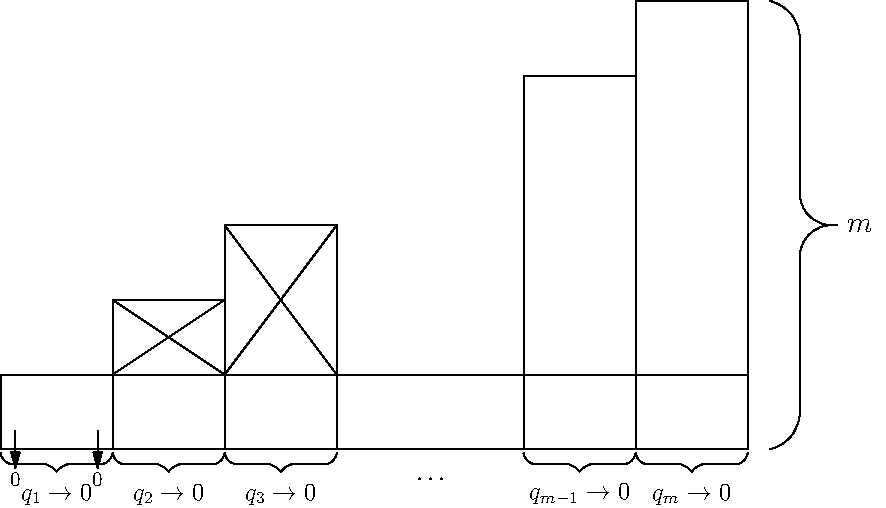
\includegraphics[width=14cm]{image/Asymptote/2/linal-2-1.pdf}
    \end{center}
    Применим оператор $B$:
    $$\begin{cases}
        \dim V = q_1 + 2q_2 + ... + (m-1)q_{m-1} + mq_m = n\\
        \dim \text{Im}B = q_2 + ... + (m-2)q_{m-1} + (m-1)q_m = r_1\\
        \vdots \\
        \dim \text{Im}B^{m-1} = q_m = r_{m-1}
    \end{cases}$$  
    Некоторые применения приведут матрицу к жордановой форме (в частности, диагонализируемости)
    \subsection{Решение СЛАУ}
    Пусть дана система $AX = B$ с квадратной матрицей $A$, все характеристические корни которой $\in \R$.\\
    Сделаем замену: 
    $$X = CY \Longrightarrow (AC)Y = B \Longleftrightarrow (\underbrace{C^{-1}AC}_{y} )Y = C^{-1}b=b'$$
    Можно взять $C$ - матрицу перехода к жорданову базису
    $$y = \begin{pmatrix}
        \text{\fbox{ $Y_{k_1}(\lambda_1)$ }} & \null & 0\\
        \null & \ddots \\
        0 & \null & \text{\fbox{$Y_{k_i}(\lambda_i)$}}
    \end{pmatrix}$$
    Если $y$ жорданова клетка, то уравнения:
    $$\begin{cases}
        \lambda x_1 + x_2 = b_1'\\
        \lambda x_2 + x_3 = b_2'\\
        \vdots
    \end{cases} \ \ \ \text{легко решить}$$
    \subsection{Решение СЛДУ}
    $$X = \begin{pmatrix}
        x_1(t)\\
        \vdots\\
        x_n(t)
    \end{pmatrix} , \ \ \frac{dx}{dt} = \begin{pmatrix}
        \dot{x}_1 \\
        \vdots\\
        \dot{x}_n
    \end{pmatrix}$$
    $\dot{X} = AX$, где $A$ - квадратная
    $$X = CY \Longrightarrow \dot{X} = C\dot{Y}$$
    $$C\dot{Y} = (AC)Y \Longrightarrow \dot{Y} = (C^{-1}AC)Y$$
    Если матрица $C^{-1}AC$ диагональная: $C^{-1}AC = \begin{pmatrix}
        \lambda_1 & \null & 0\\
        \null & \ddots & \\
        0 & \null & \lambda_n
    \end{pmatrix}, \ \lambda_i \neq 0$ получаем систему: 
    $$\begin{cases}
        \dot{y_1} = \lambda_1 y_1\\
        \vdots \\
        \dot{y_n} = \lambda_n y_n
    \end{cases} \Longrightarrow \begin{cases}
        y_1 = C_1e^{\lambda_1t}\\
        \vdots \\
        y_n = C_ne^{\lambda_nt}
    \end{cases}$$
    Тогда $X = CY$\\
    Если $$C^{-1}AC = J_k(\lambda_0) = \begin{pmatrix}
        \lambda_0 & 1 & \null & 0 \\
        \null & \ddots & \ddots & \null \\
        \null & \null & \lambda_{0} & 1 \\
        0 & \null & 0 & \lambda_0
    \end{pmatrix} \Longrightarrow \begin{cases}
        \dot{y}_1 = \lambda_0y_1 + y_2\\
        \vdots \\
        \dot{y}_{n-1} = \lambda_0y_{n-1} + y_n\\
        \dot{y}_n = \lambda_0y_n
    \end{cases}$$
    решаем снизу вверх.
    \subsection{Функции от матриц}
    %$\underset{n \in \N}{A^n}$ 
    $$(C^{-1}AC) = J = \begin{pmatrix}
        \text{\fbox{ $J_{k_1}(\lambda_1)$ }} & \null & 0\\
        \null & \ddots \\
        0 & \null & \text{\fbox{$J_{k_i}(\lambda_i)$}}
    \end{pmatrix} \Longrightarrow A = CYC^{-1}$$ 
    $$\Longrightarrow A^n = (CYC^{-1})(CYC^{-1})...(CYC^{-1}) = CY^nC^{-1}$$
    $$J^n = \begin{pmatrix}
        \text{\fbox{ $J_{k_1}^n(\lambda_1)$ }} & \null & 0\\
        \null & \ddots \\
        0 & \null & \text{\fbox{$J_{k_i}^n(\lambda_i)$}}
    \end{pmatrix}$$
    Для жордановой клетки: 
    $$\left(\begin{smallmatrix}
        \lambda_1 & 1 & \null & 0 \\
        \null & \ddots & \ddots & \null \\
        \null & \null & \lambda_{n-1} & 1 \\
        0 & \null & 0 & \lambda_n 
    \end{smallmatrix}\right)^n = \left(\lambda E + \left(\begin{smallmatrix}
        0 & 1 & \null & 0 \\
        \null & \ddots & \ddots & \null \\
        \null & \null & 0 & 1 \\
        0 & \null & 0 & 0 
    \end{smallmatrix}\right)\right) =$$ 
    $$= \lambda^n E + C_n^1 \lambda^{n-1}B + C_n^2 \lambda^{n-2}B^2 + ... = \begin{pmatrix}
        \lambda^n & \lambda^{n-1}C_n^1 & \lambda^{n-2}C_n^2 & \cdots\\
        \tab[1cm] \ddots & \tab[1cm] \ddots & \tab[1cm] \ddots \\
        \null & \lambda^n & \lambda^{n-1}C_n^1 & \lambda^{n-2}C_n^2\\
        \tab[1cm] \null & \tab[1cm] \ddots \\
        \null & \null & \lambda^n 
    \end{pmatrix}$$
    \begin{exercise}
        Пусть $f(t)$ - многочлен, \ $J = \left(\begin{smallmatrix}
            \lambda & 1 & \null & 0\\
            \null & \ddots & \ddots\\
            \null & \null & \ddots & 1 \\
            0 & \null & \null & \lambda
        \end{smallmatrix}
        \right)$\\
        Доказать, что:
        $$f(J) = \begin{pmatrix}
            f(\lambda) & f'(\lambda) & \frac{f''(\lambda)}{2!} & \cdots\\
            \null & \ddots \\
            \null & \null & \ddots\\
            \null & \null & \null & \ddots\\
            \null & \null & \null & \null & f(\lambda)
        \end{pmatrix}$$  
    \end{exercise}
    \subsection{Вычисление корня и экспоненты}
    $$e^{at} = 1 + \frac{at}{1!} + \frac{a^2t^2}{2!} + ... + \frac{a^{n-1}t^{n-1}}{(n-1)!} + ...$$
    $$e^{At} = E + \frac{At}{1!} + \frac{A^2t^2}{2!} + ... + \frac{A^{n-1}t^{n-1}}{(n-1)!} + ...$$
    Для $J_n(\lambda) = \lambda E + B \Longrightarrow$ 
    $$\exp (J_n(\lambda)t) = e^{t \lambda E} \cdot e^{tB} = e^{\lambda t}\cdot \begin{pmatrix}
        1 & t & \frac{t^2}{2} & \cdots\\
        \null & 1 & t & \frac{t^2}{2}\\
        \null & \null & \ddots & \ddots & \ddots\\
        \null & \null & \null & \ddots & \ddots & \null\\
        \null & 0 & \null & \null & \ddots \\
        \null & \null & \null & \null & \null & 1
    \end{pmatrix}
    $$
    $$(e^{A + B} = e^A \cdot e^B \Longleftrightarrow AB = BA)$$
    \begin{example}\tab
        \begin{enumerate}
            \item $$(1 + t)^{\frac{1}{2}} = 1 + \frac{1}{2}t +      \frac{1}{2!}\cdot \frac{1}{2}\cdot(\frac{1}{2}-1)t^2 + ...$$
            \item $$\begin{pmatrix}
            \lambda & 1 \\
                0 & \lambda
                \end{pmatrix} = E + \frac{1}{2}B + \frac{1}{2!}C^2_{\frac{1}{2}}B^2 = \begin{pmatrix}
                1 & \frac{1}{2} \\
                0 & 1
                \end{pmatrix}$$
            \item $$\begin{pmatrix}
                    \lambda & 1 \\
                    0 & \lambda
                \end{pmatrix} = \lambda^{\frac{1}{2}} \cdot \begin{pmatrix}
                    1 & \frac{1}{\lambda} \\ 0 & 1
                \end{pmatrix}^{\frac{1}{2}} = \lambda^{\frac{1}{2}} \cdot \begin{pmatrix}
                    1 & \frac{1}{2\lambda} \\
                    0 & 1
                \end{pmatrix},  \ \lambda \neq 0$$
        \end{enumerate}
    \end{example}

    
    
    